\chapter{Anhang}\label{app:Anhang}

\section{Agenda der neunzehnten Acadamic Mainframe Consortium e.V. Tagung vom 16.01.2020 bis 17.01.2020}\label{app:AMC}
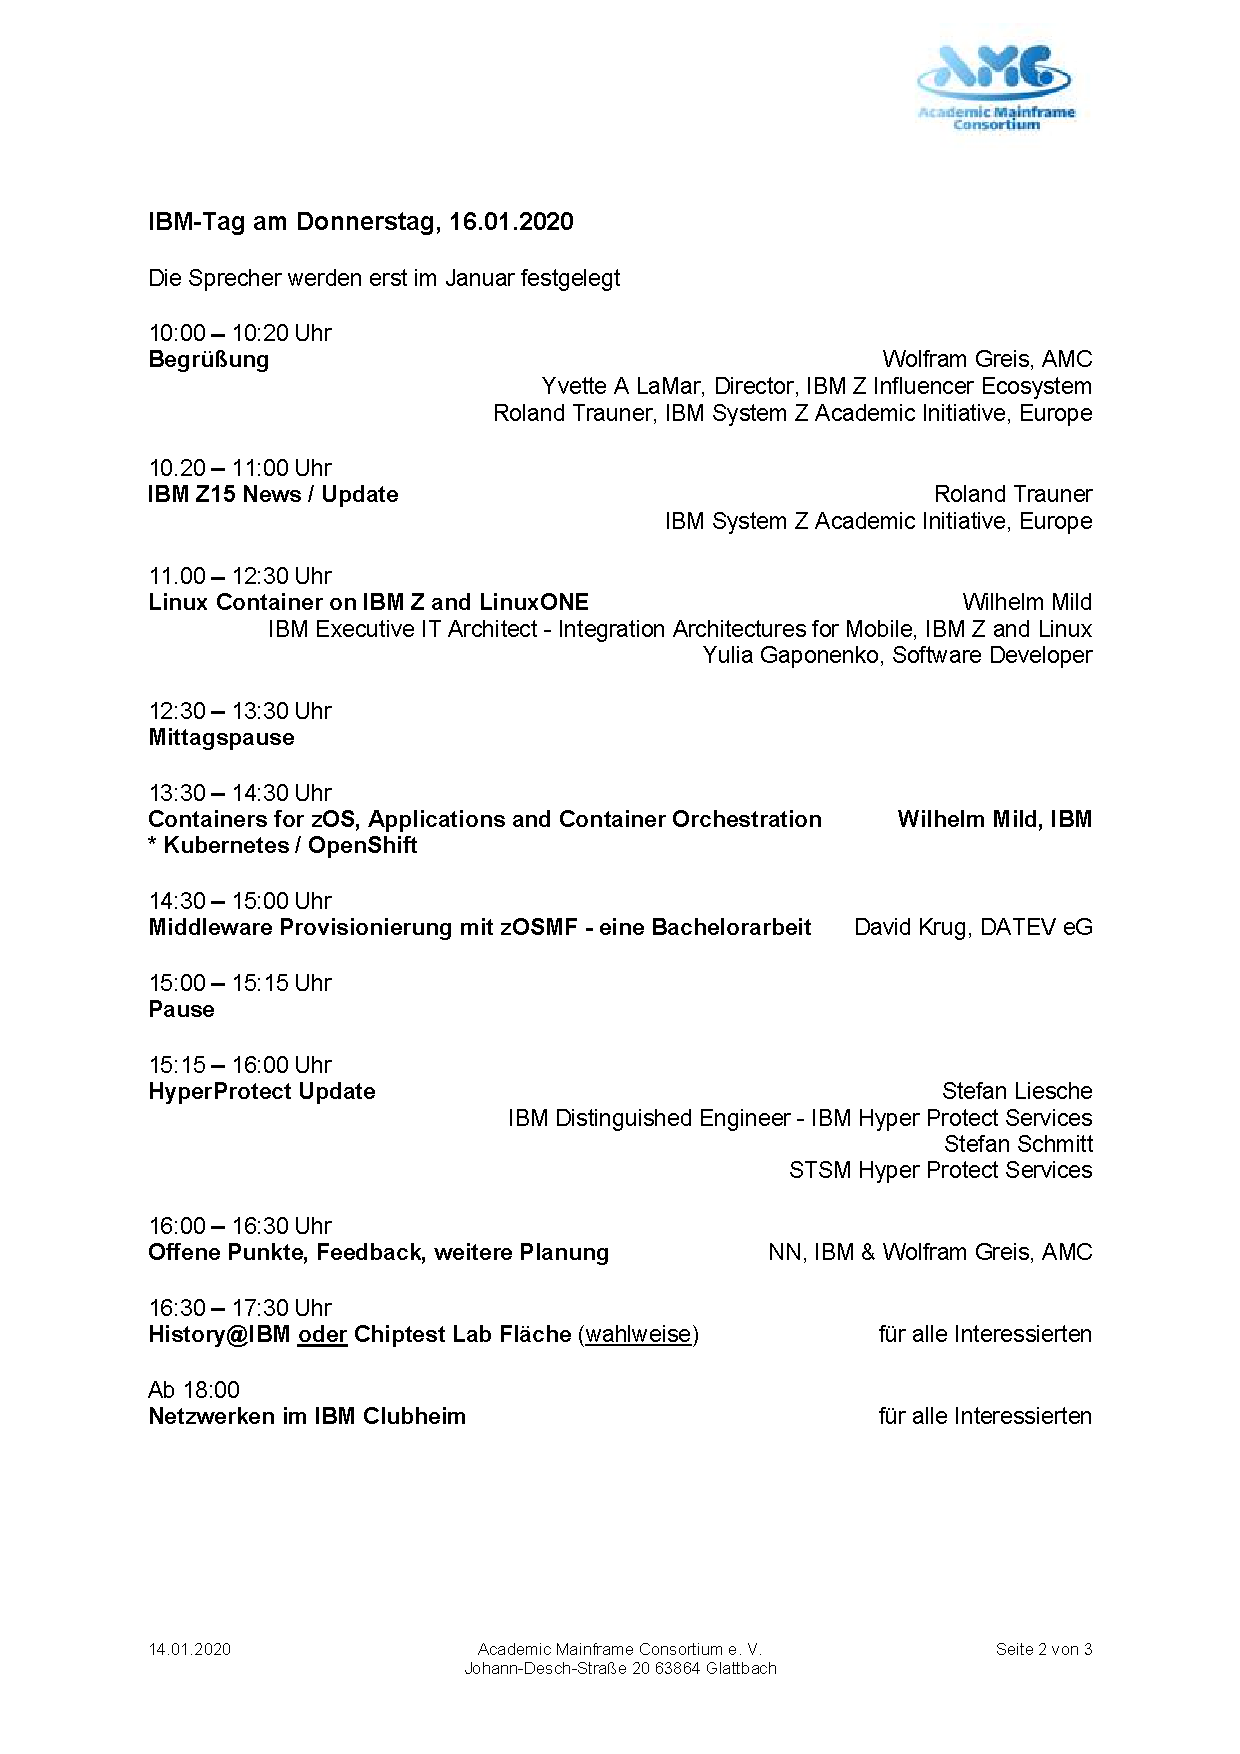
\includepdf[pages={1-}]{pdfs/AMCTagung.pdf}

\section{IT workload distribution worldwide in 2018 and 2020, by cloud type}
\begin{figure}[ht!]
\centering
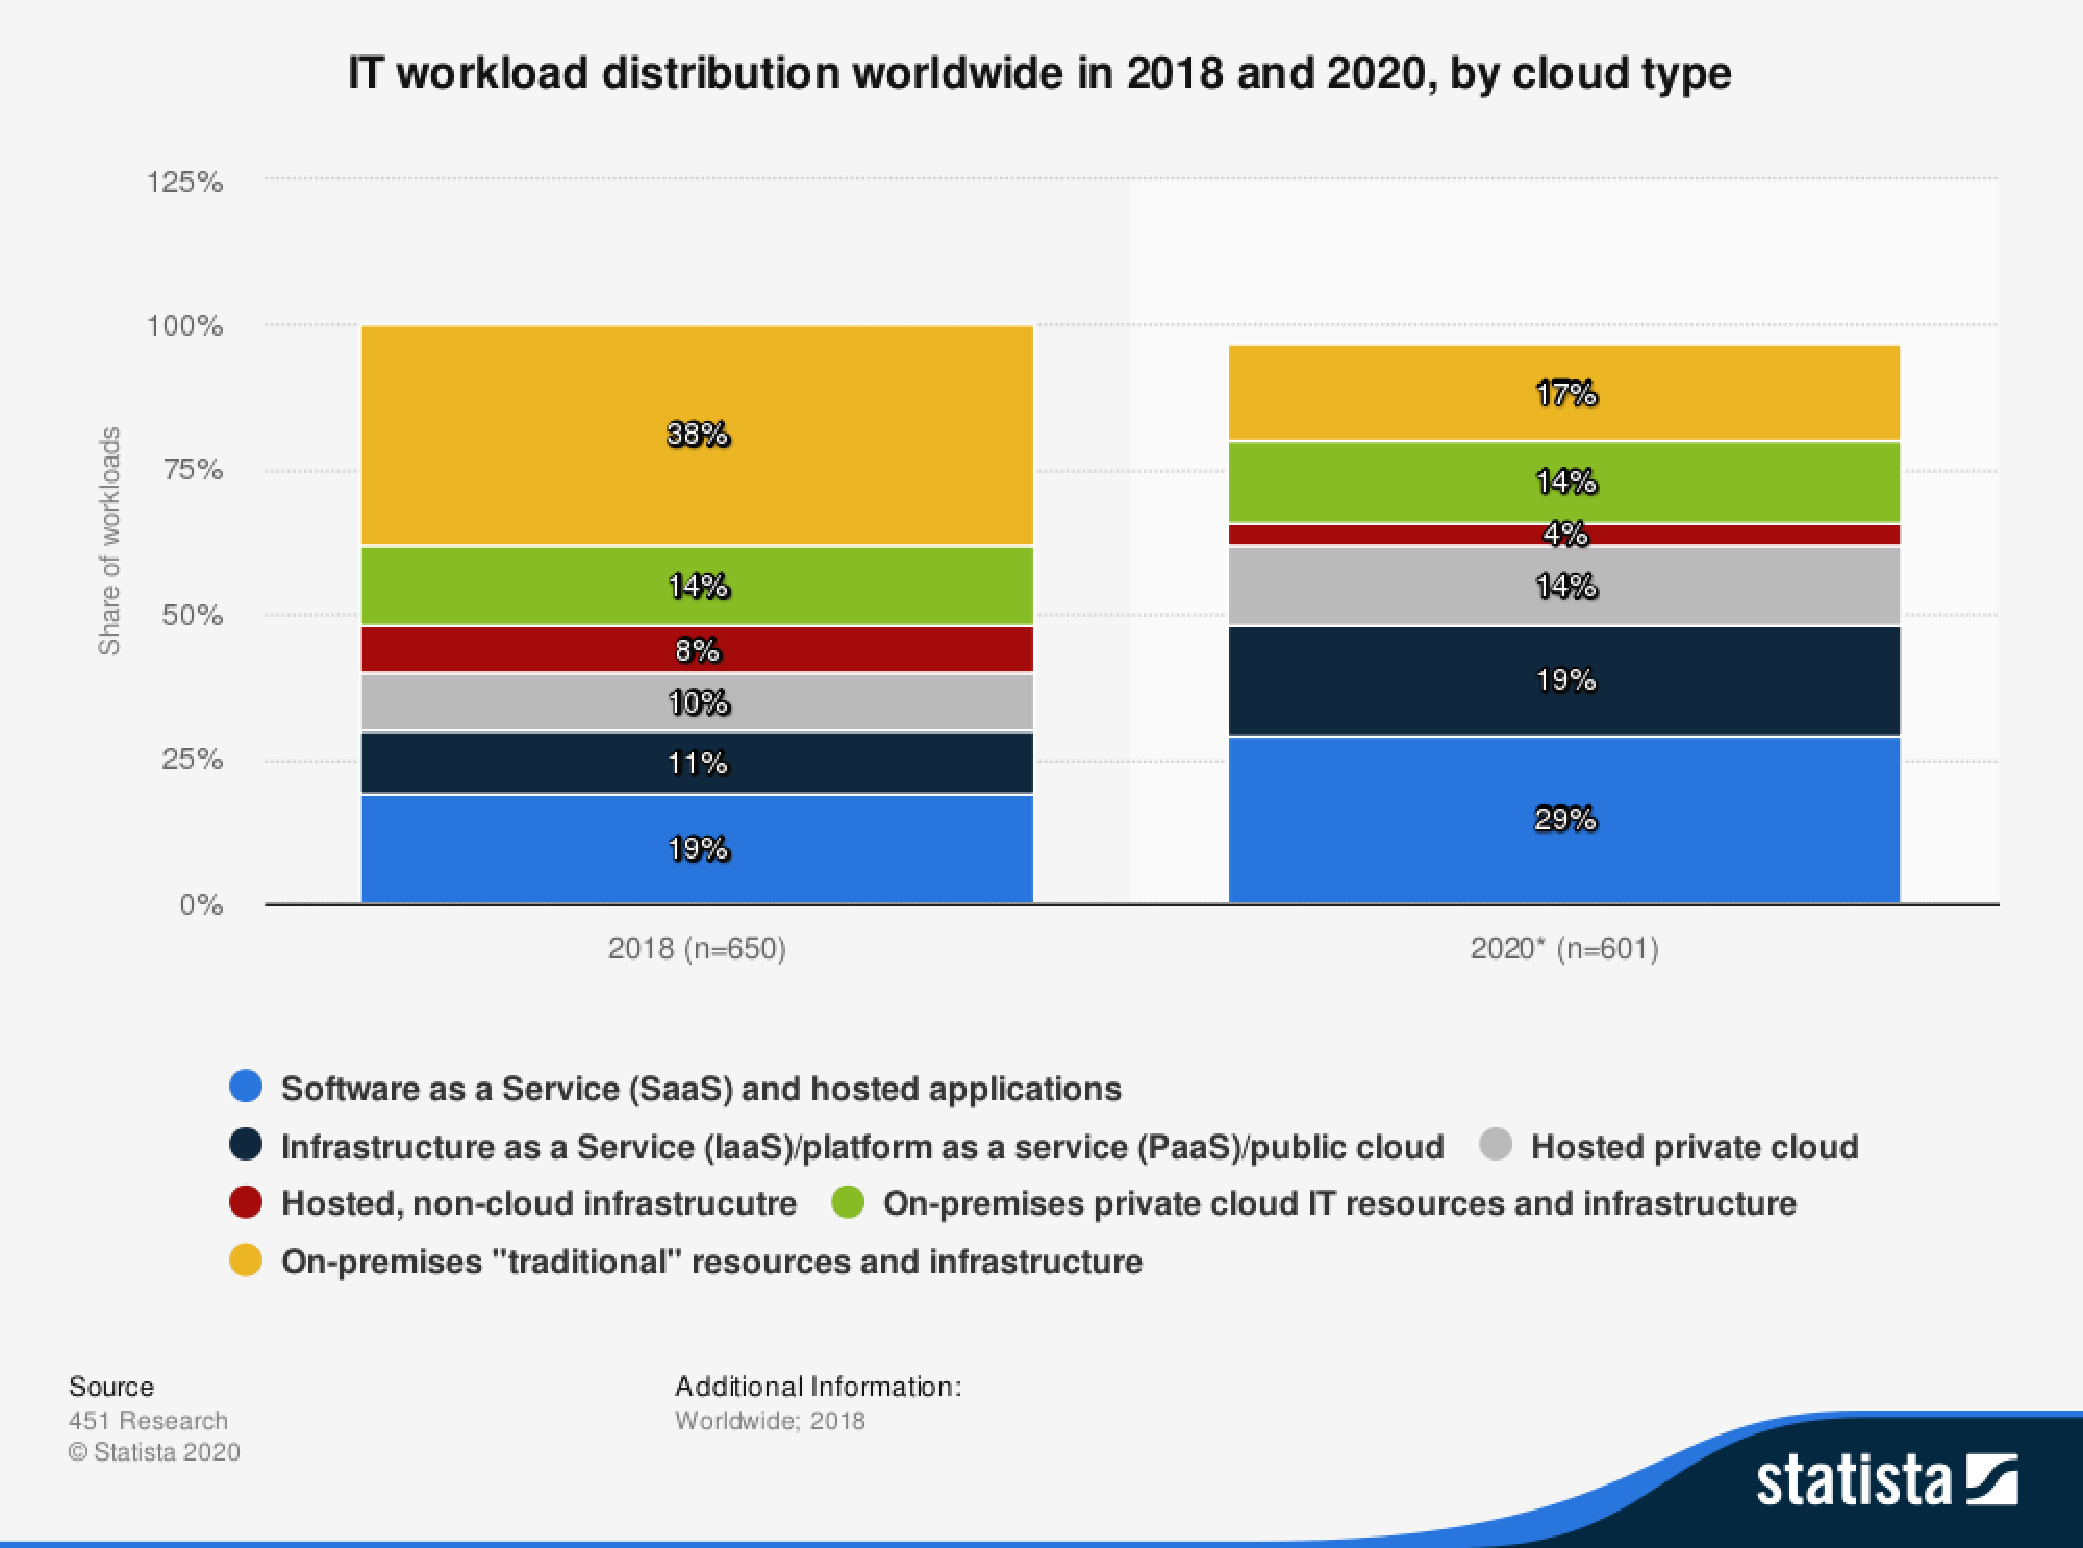
\includegraphics[width=\textwidth]{figures/statistic_id748238_it-workload-distribution-globally-2018-and-2020-by-cloud-type.pdf}
\caption{Weltweiter It Workload im Jahr 2018 und als Vorhersage im Jahr 2020 bei Cloudtyp }
\label{app:itworkload}
\end{figure}

\section{Fragen an die IBM}\label{app:ibm}
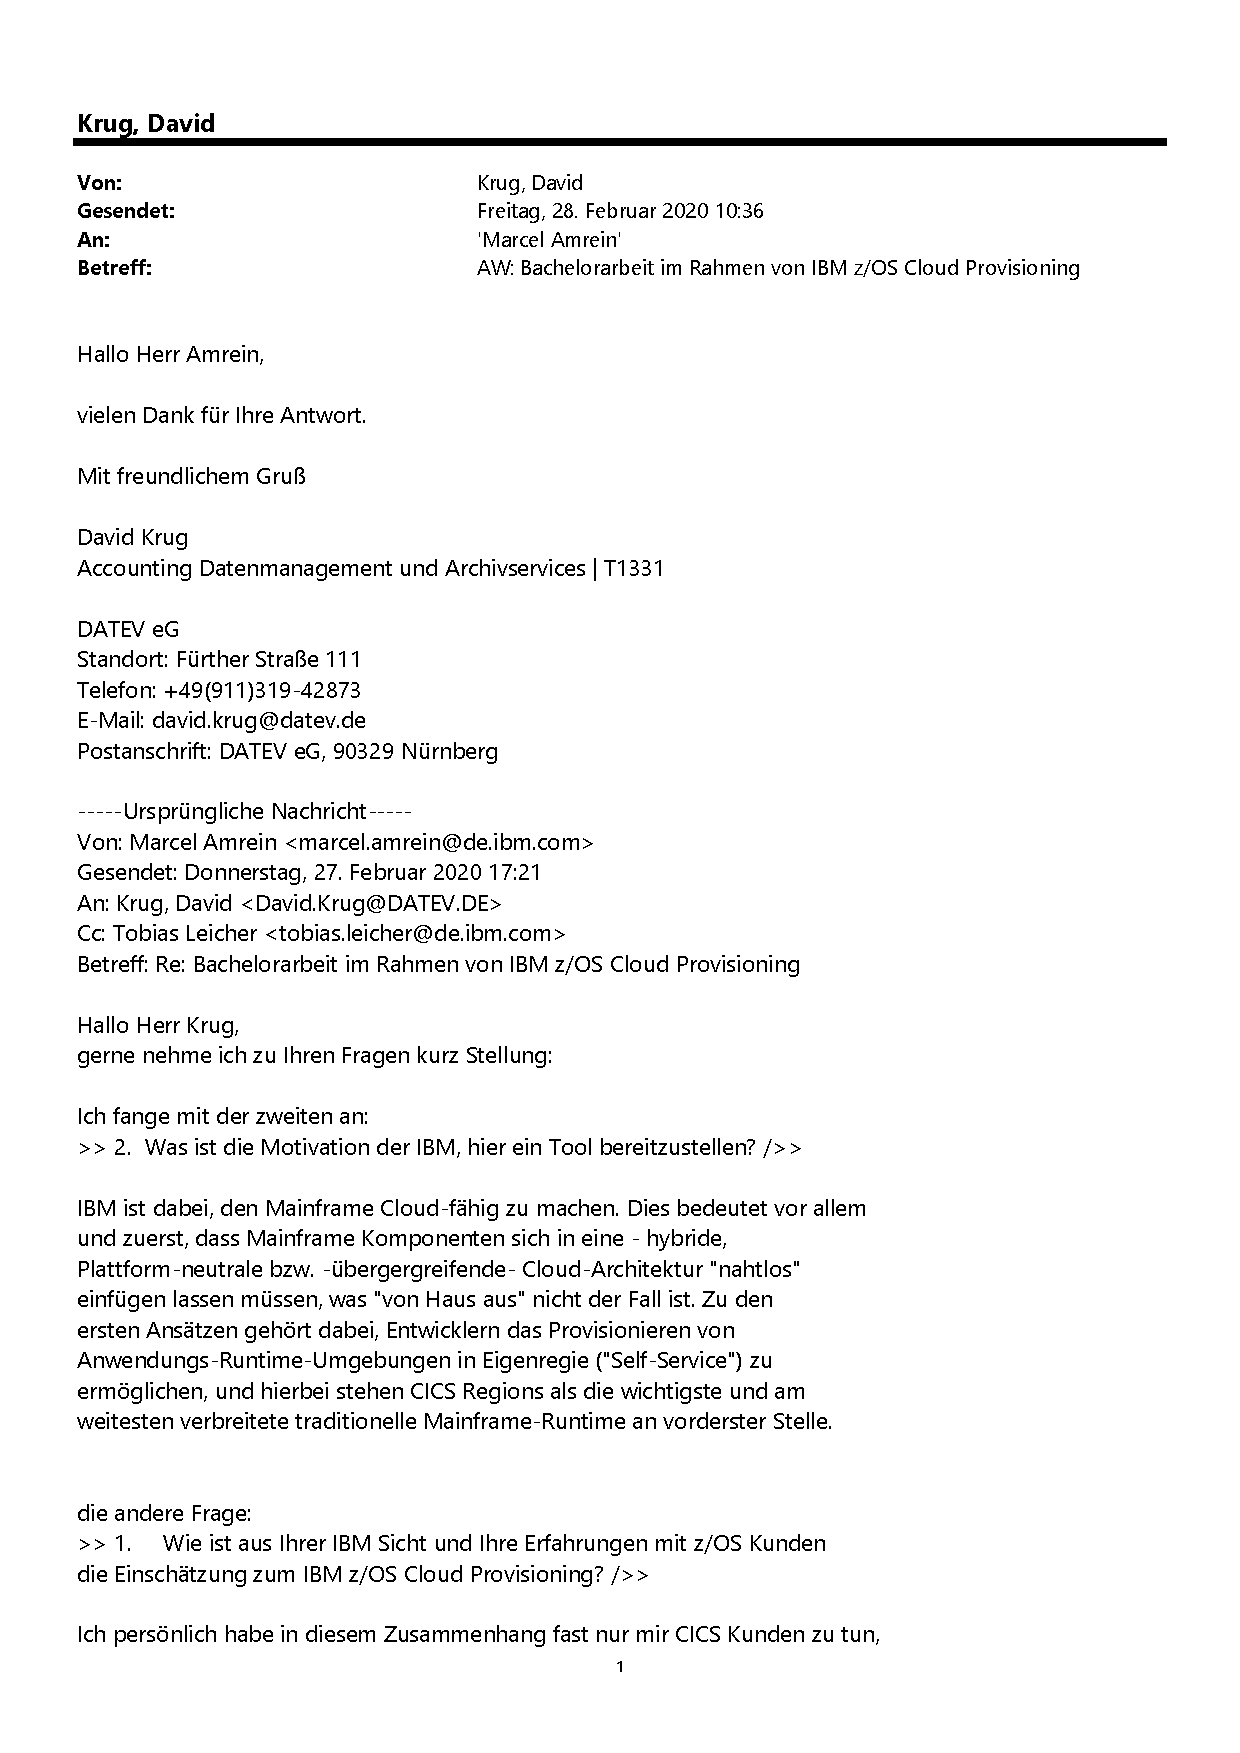
\includepdf[pages={1-}]{pdfs/MarcelMail.pdf}
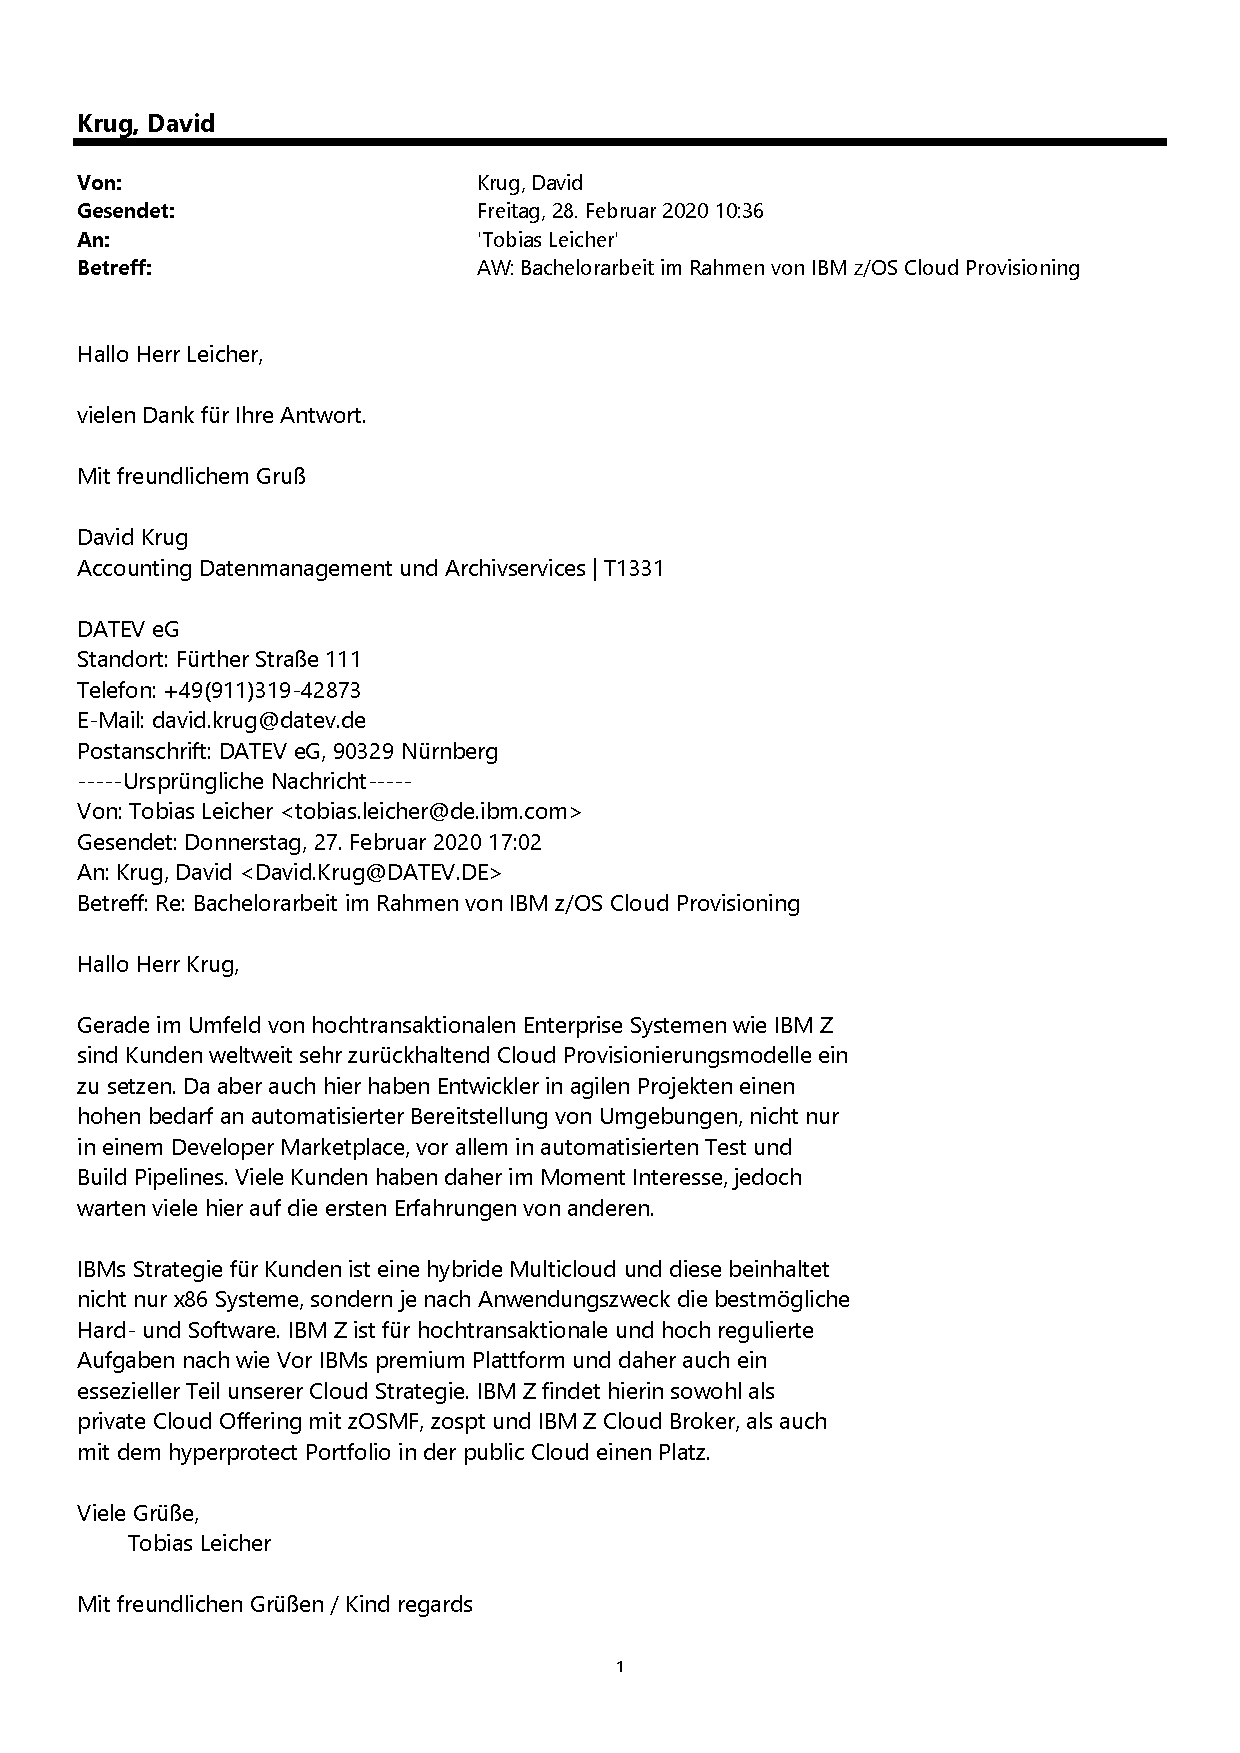
\includepdf[pages={1-}]{pdfs/TobiasMail.pdf}

\section{Interview Fragebögen}\label{app:fragen}
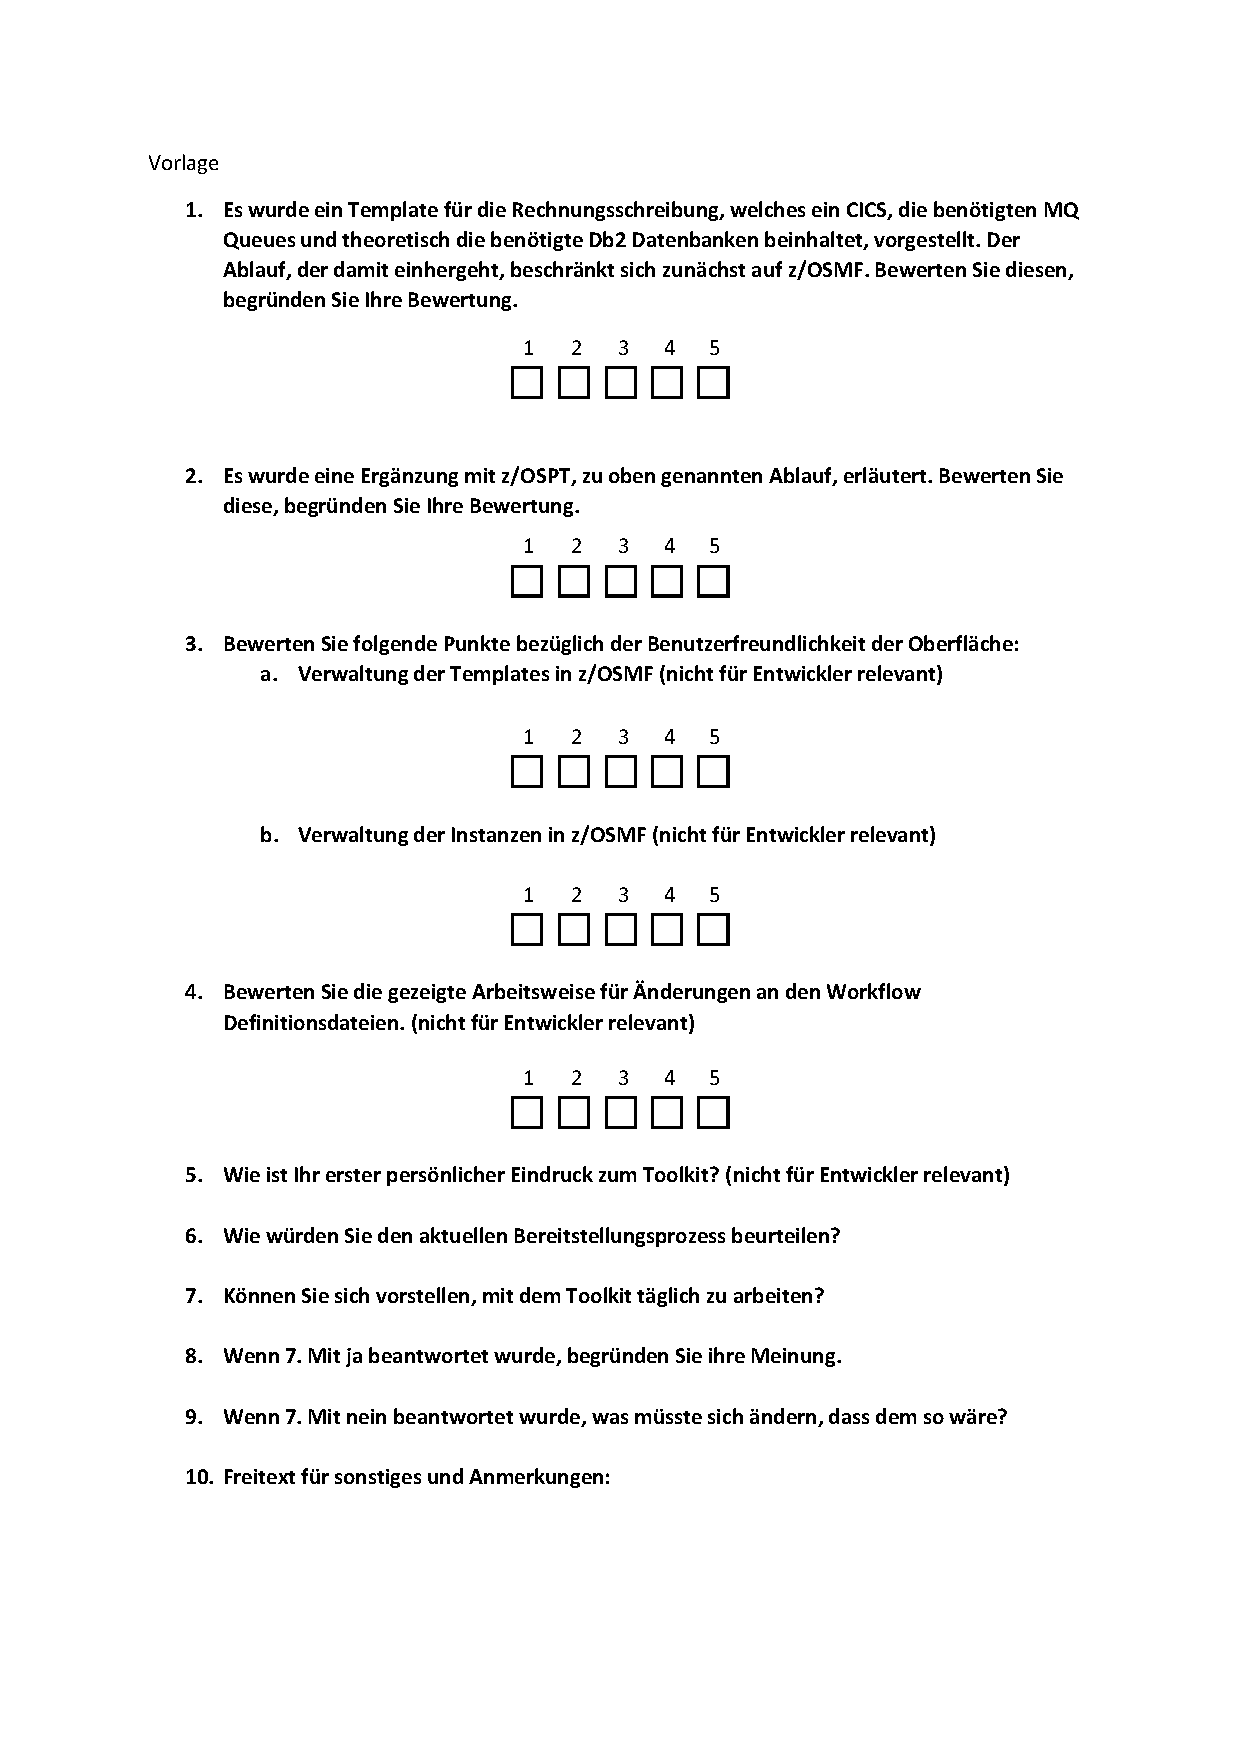
\includepdf[]{pdfs/Vorlage.pdf}
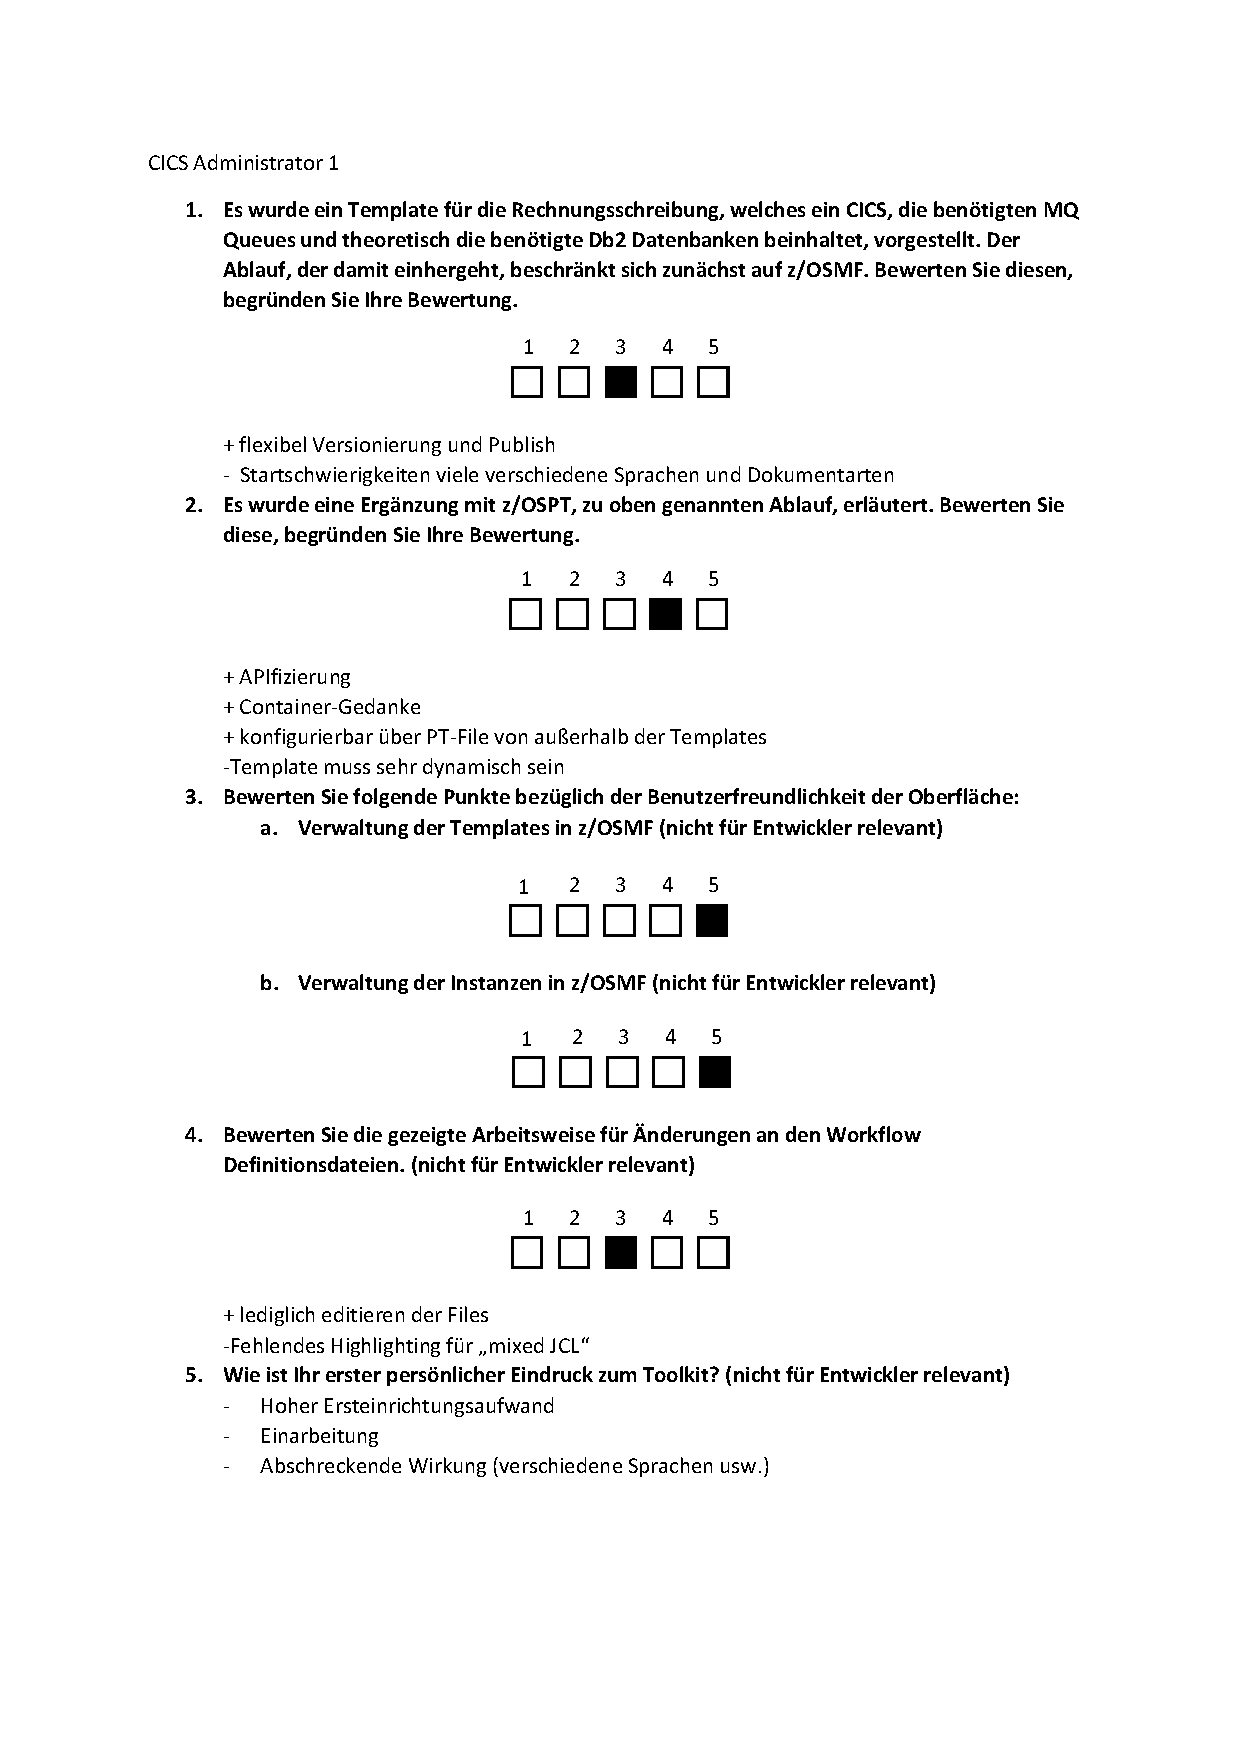
\includepdf[]{pdfs/CICSAdmin1.pdf}
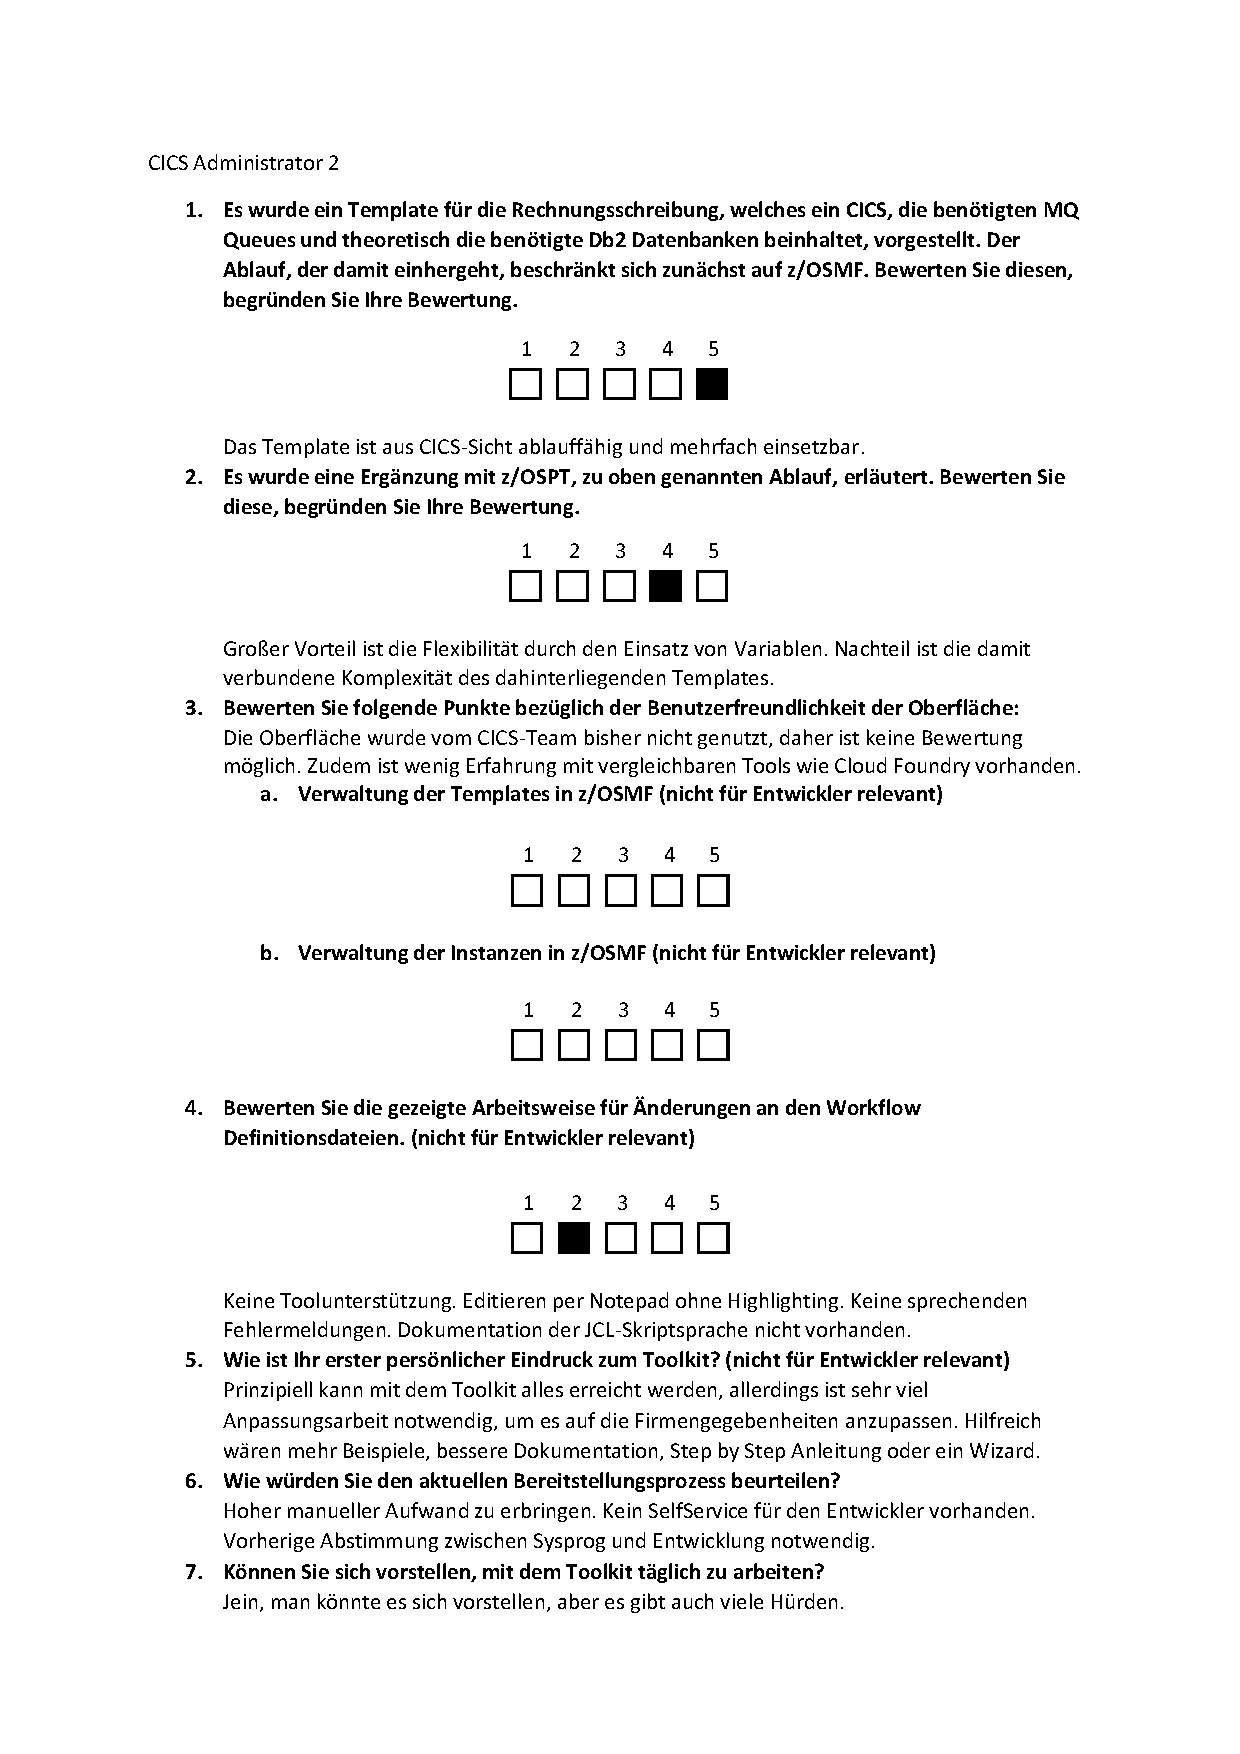
\includepdf[]{pdfs/CICSAdmin2.pdf}
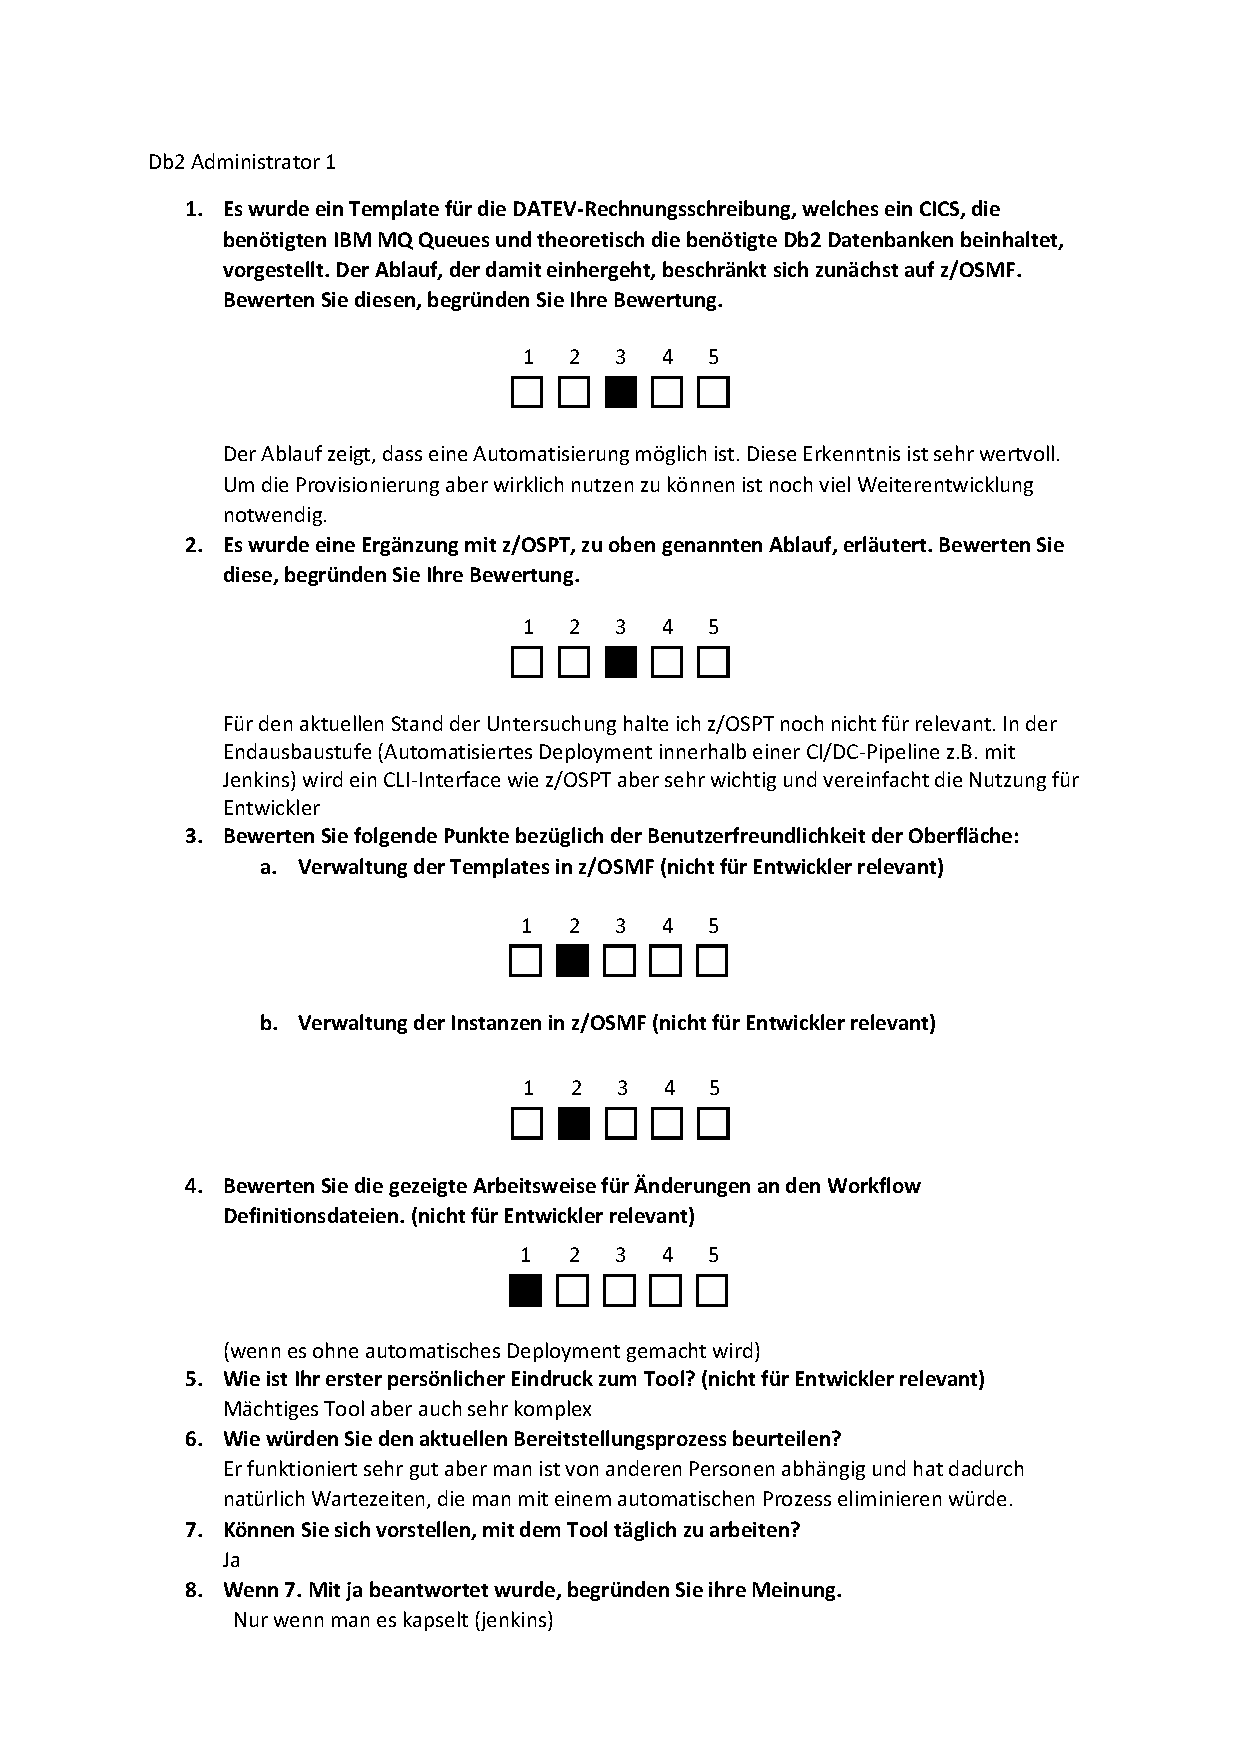
\includepdf[]{pdfs/Db2Admin1.pdf}
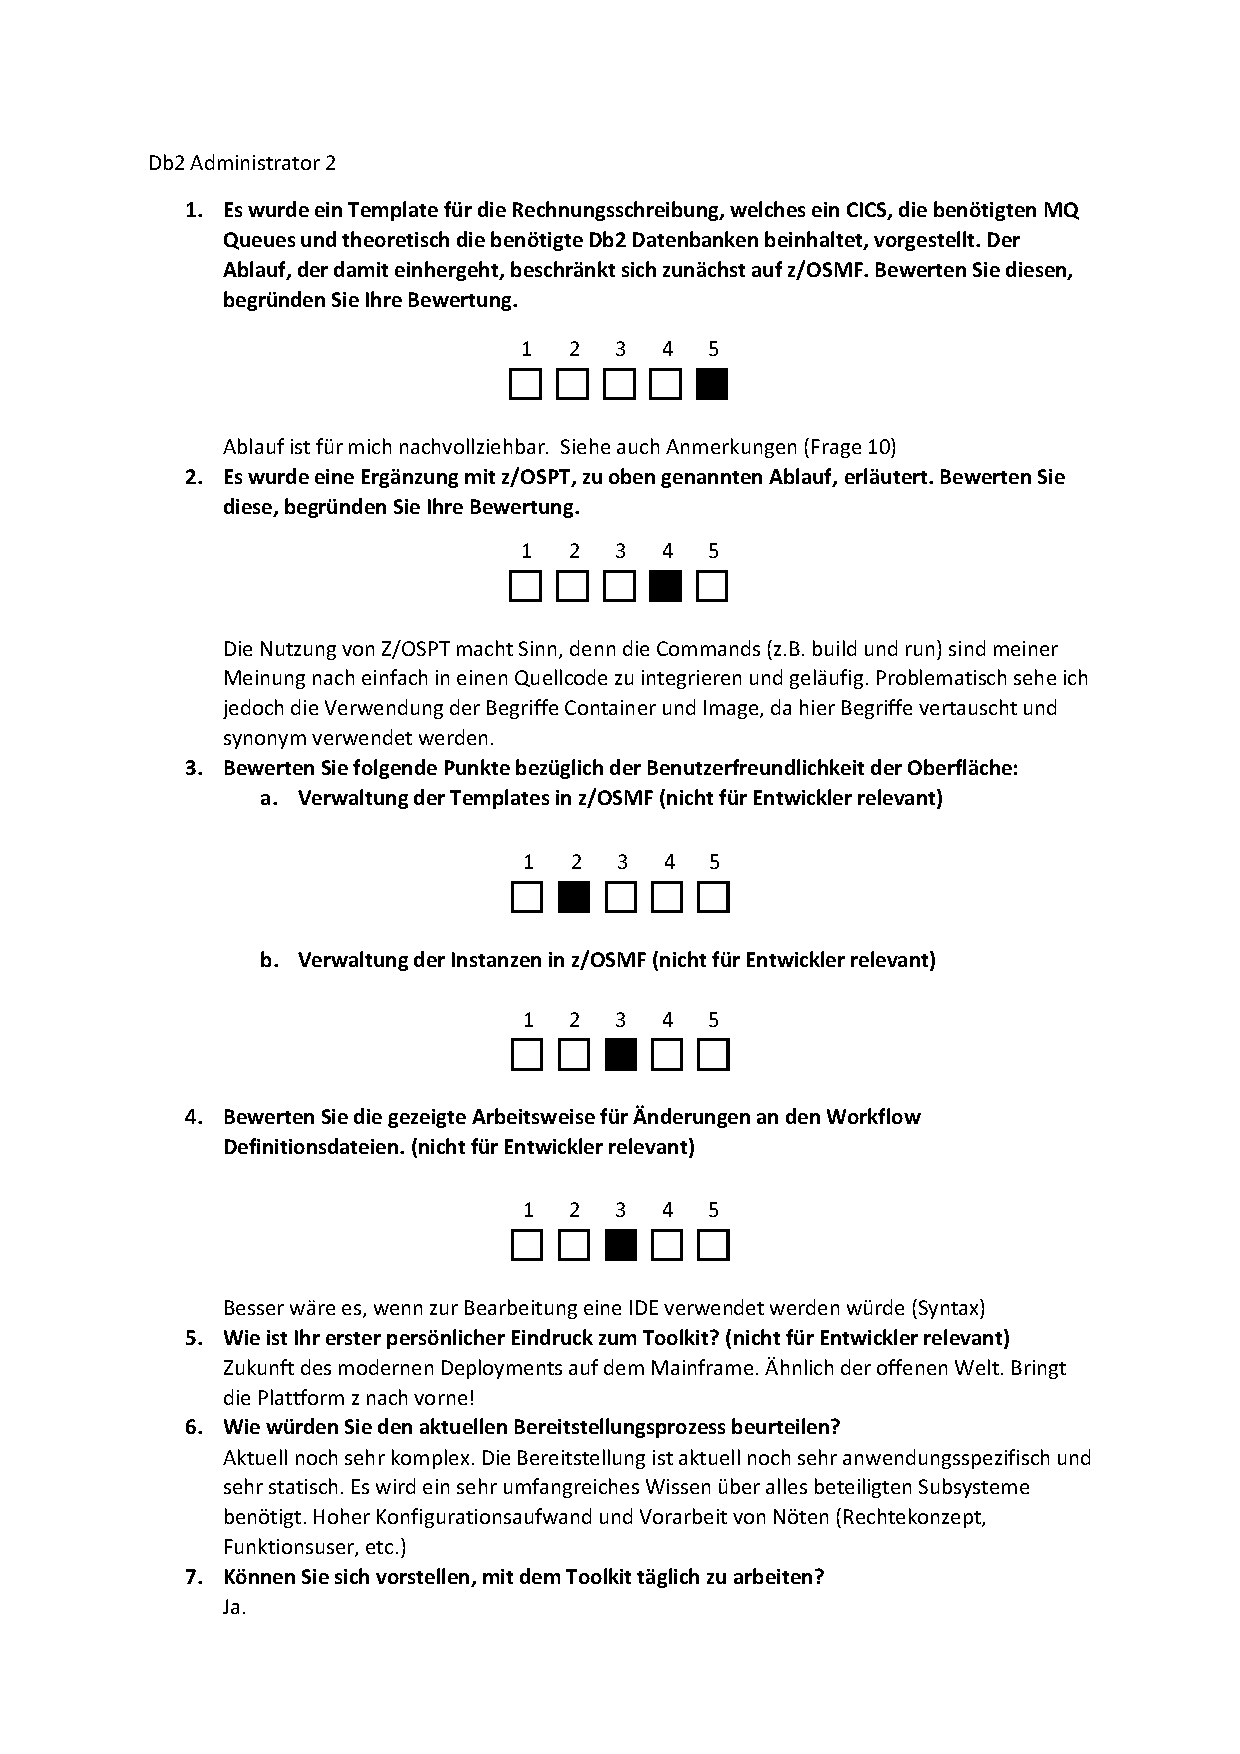
\includepdf[]{pdfs/Db2Admin2.pdf}
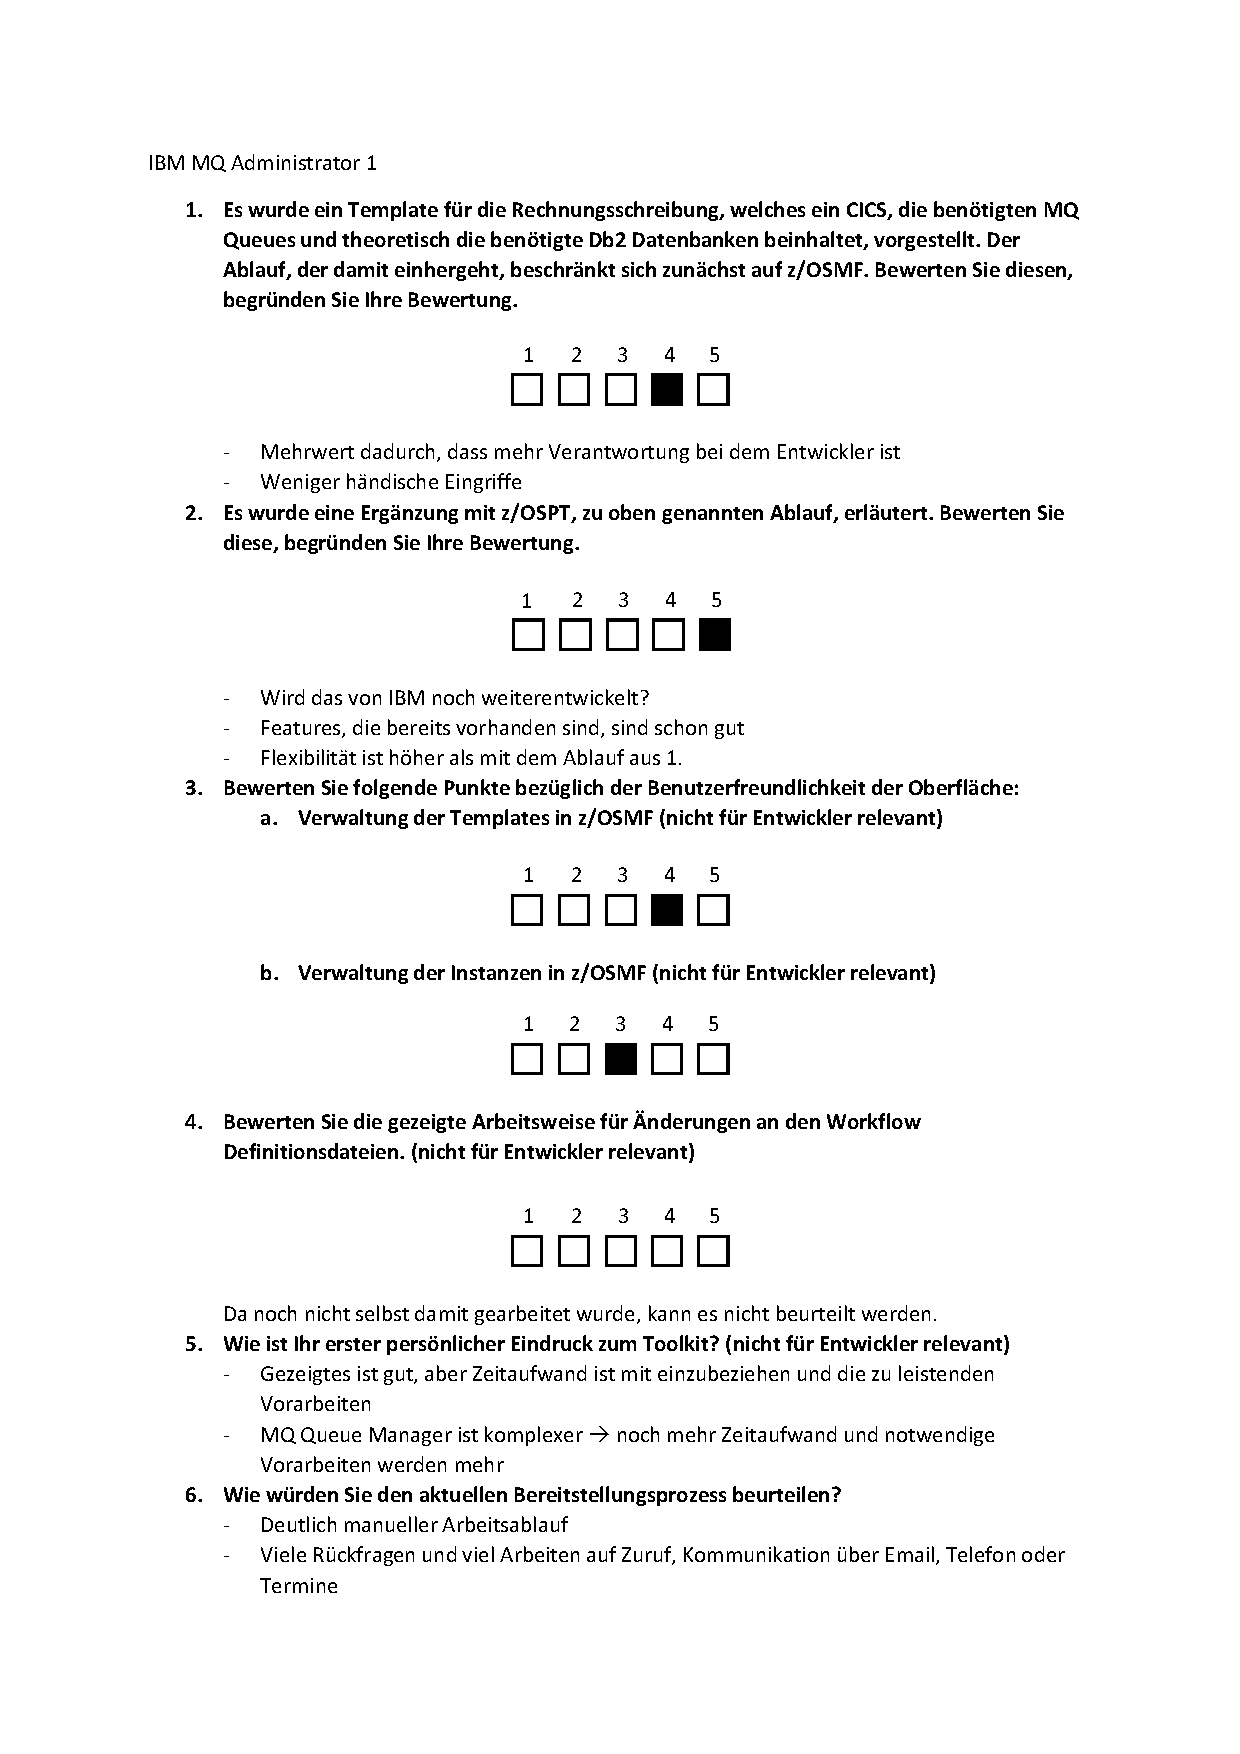
\includepdf[]{pdfs/MQAdmin1.pdf}
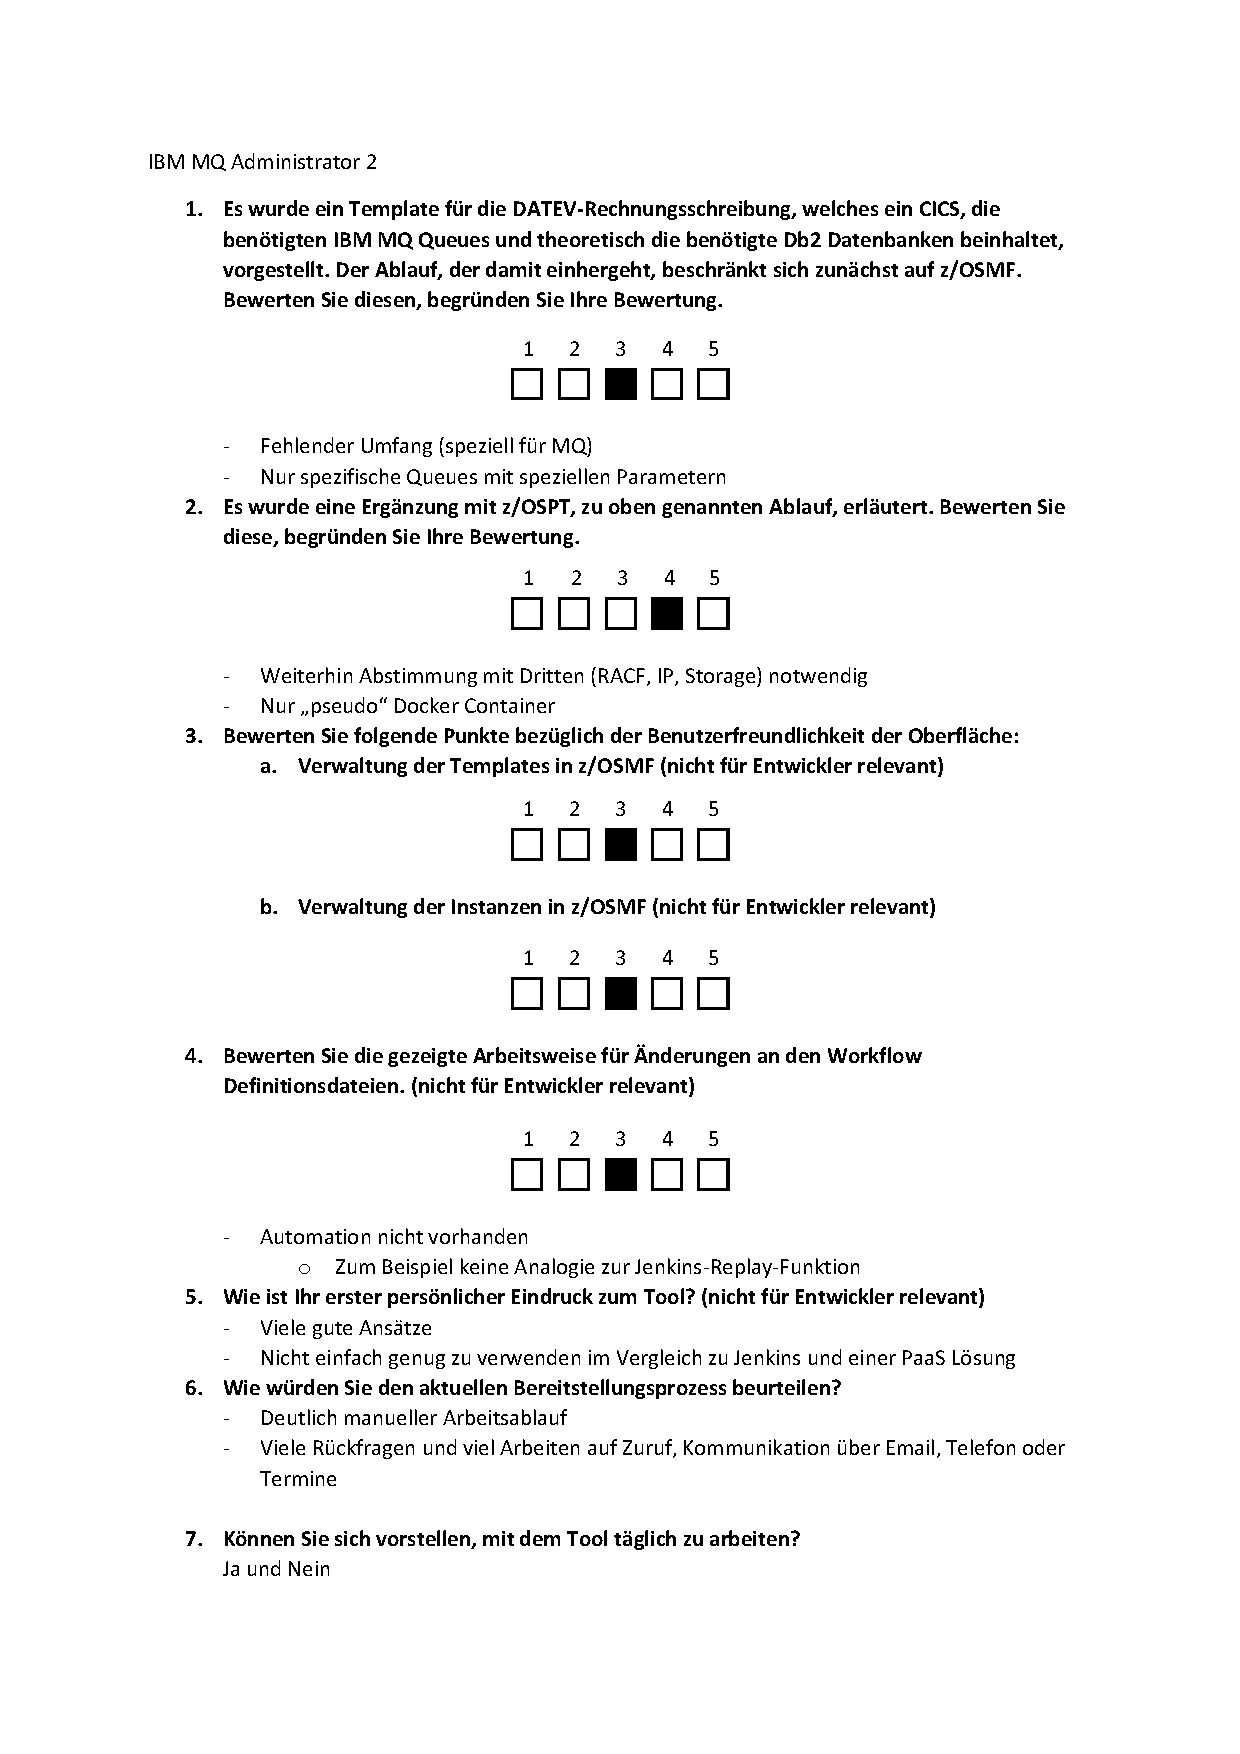
\includepdf[]{pdfs/MQAdmin2.pdf}
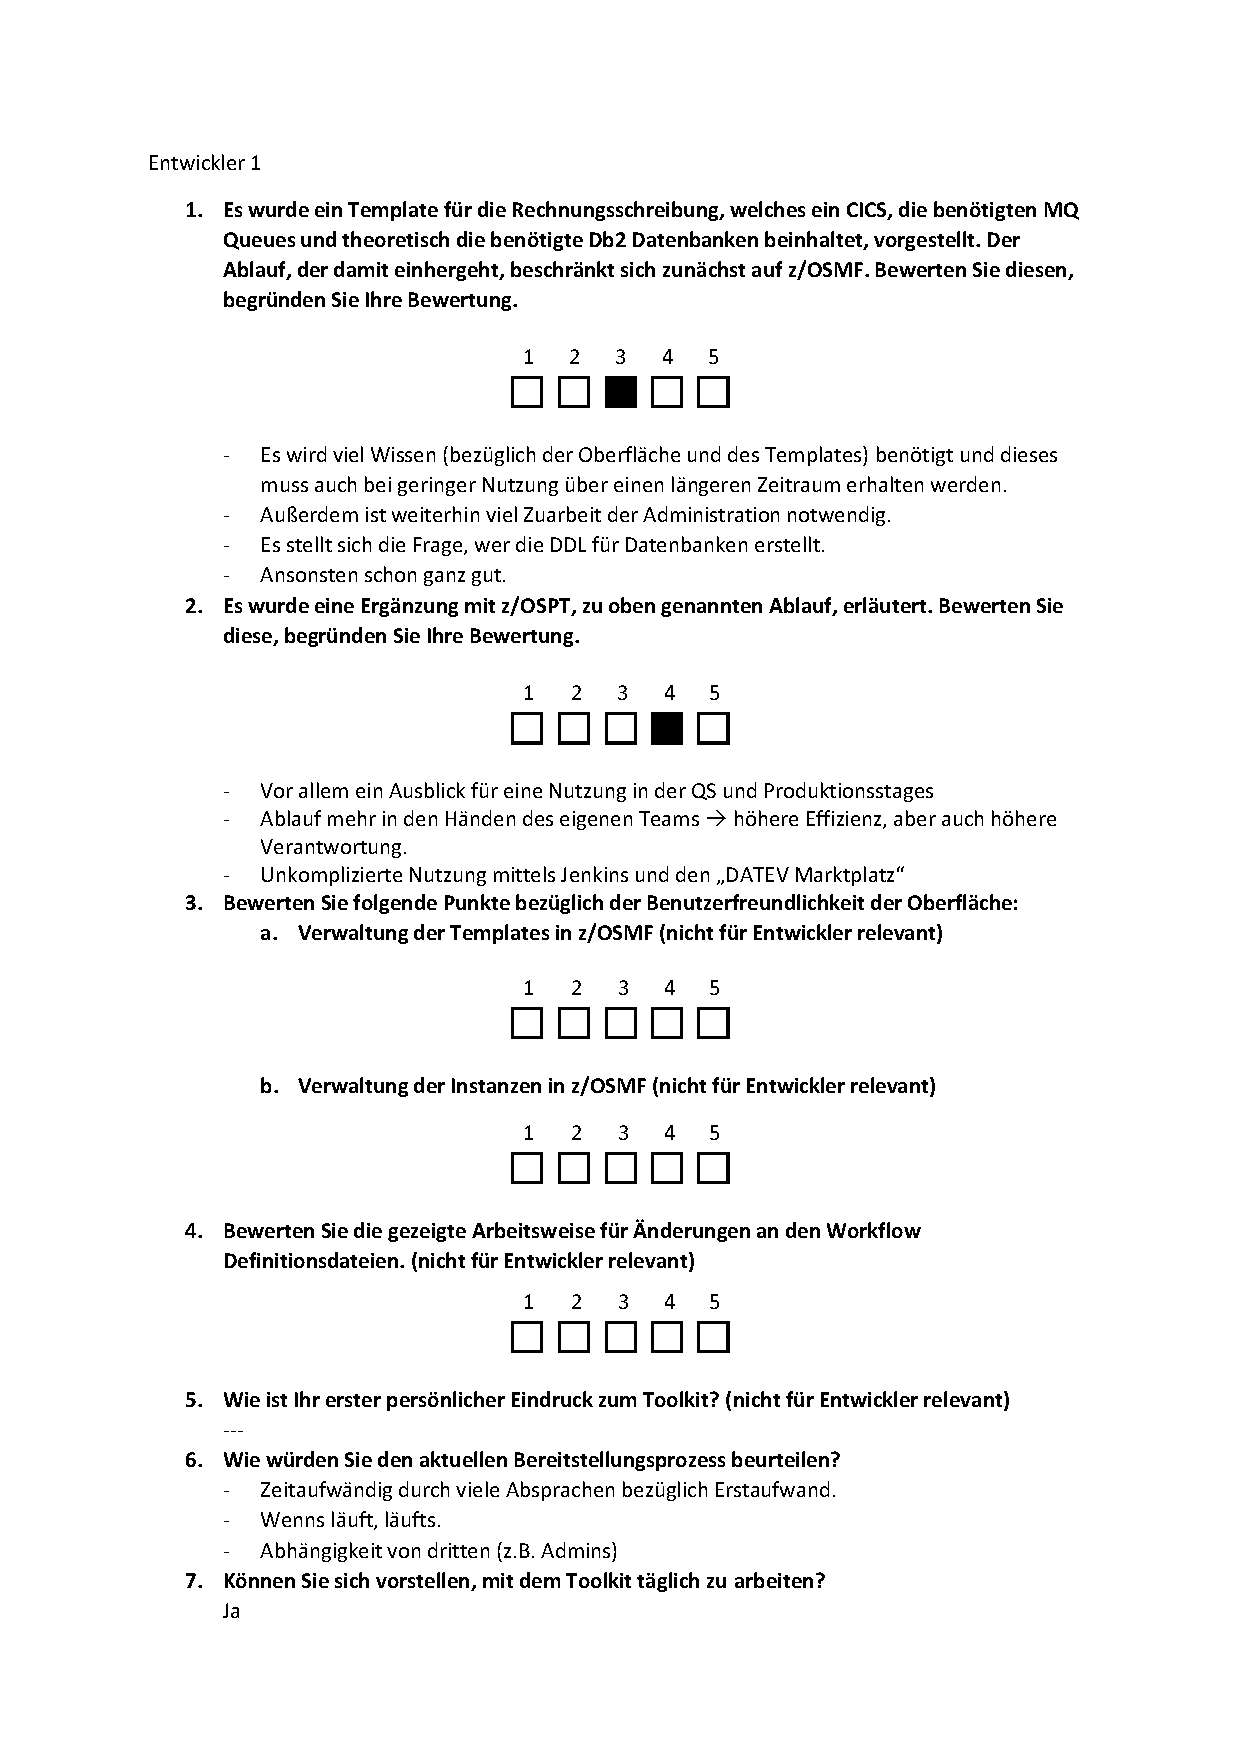
\includepdf[]{pdfs/Entwicklerteam.pdf}
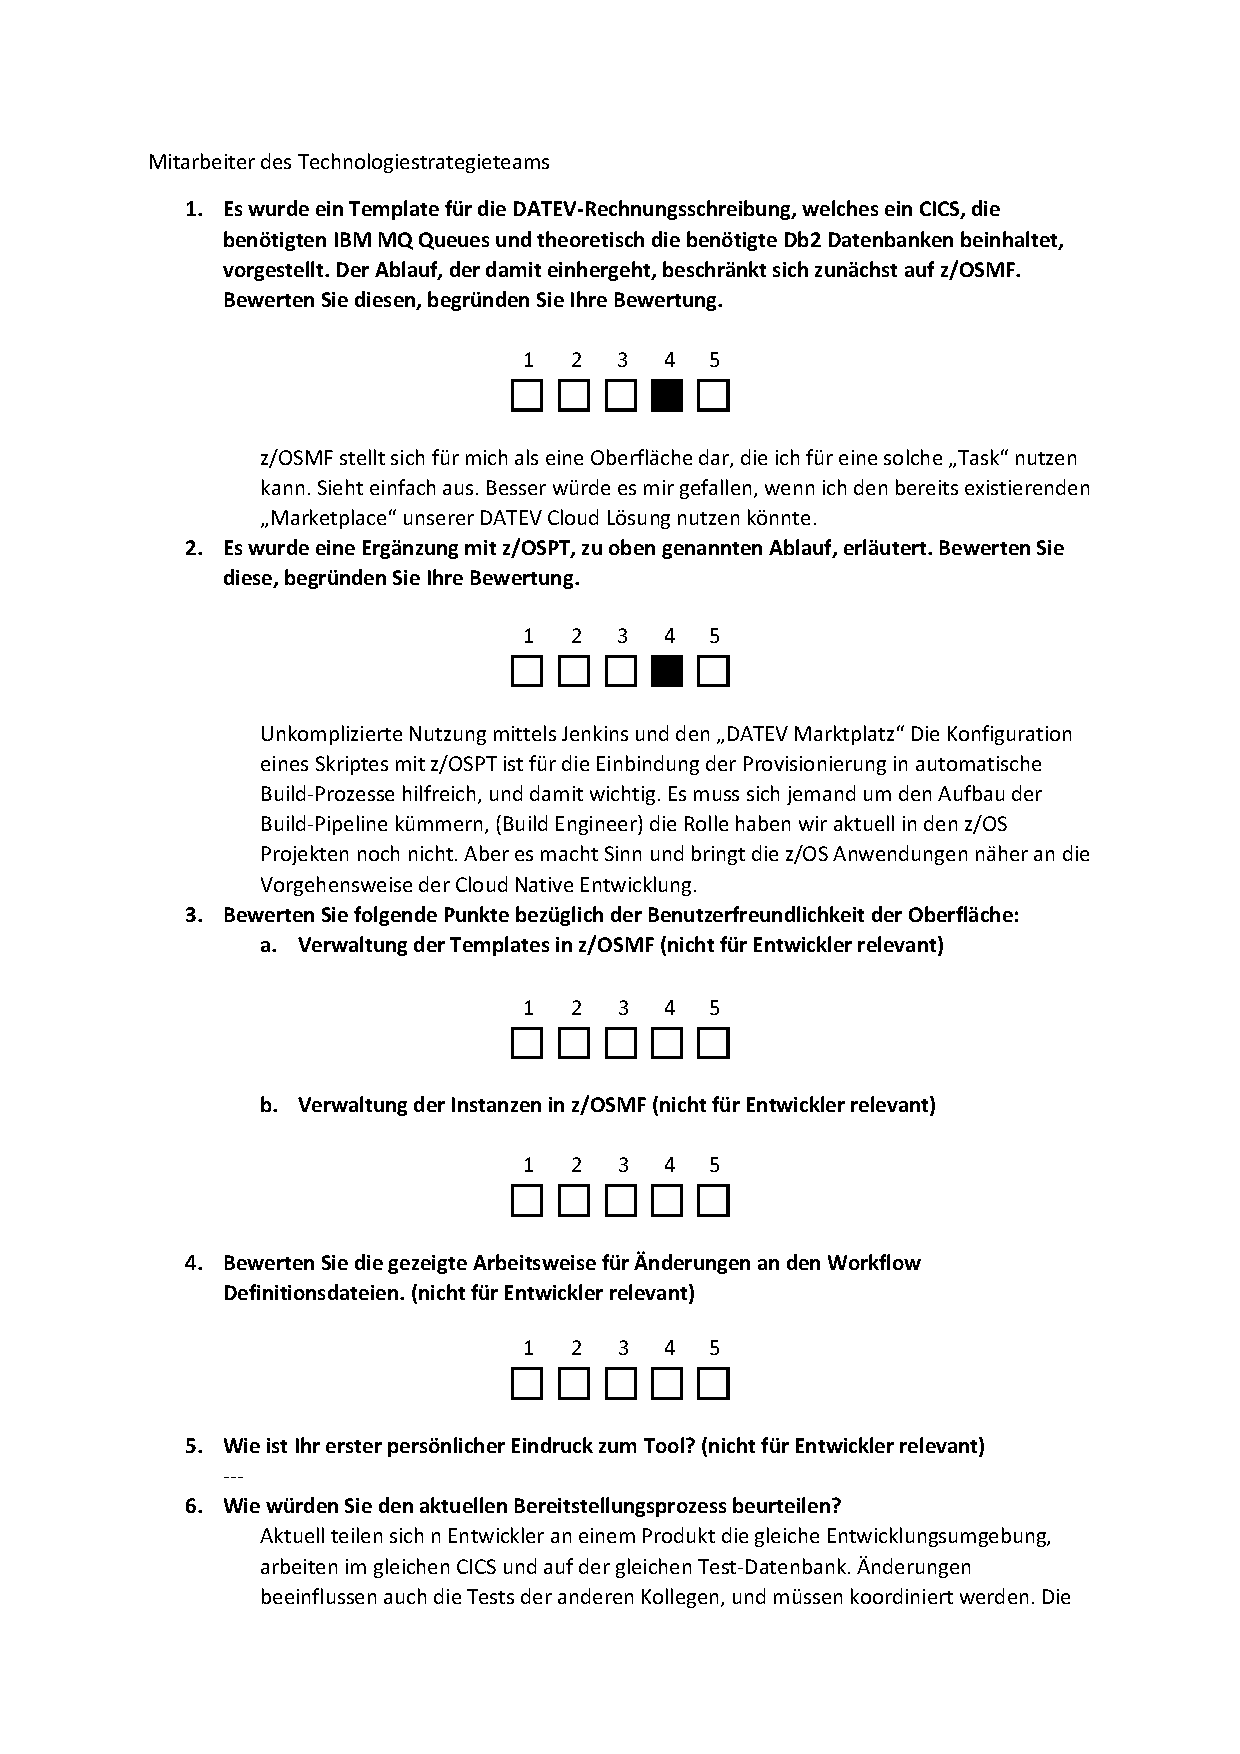
\includepdf[]{pdfs/Technologiestrategie.pdf}

\section{Workflow Step mit REST-Call}\label{app:db2prov}
\lstinputlisting[language=XML,caption{Workflow Step mit REST-Cal},captionpos=b]{listings/db2provision.xml}

\section{Produktstammdaten Tabellen Data Definition Language}\label{app:ddl}
\lstinputlisting[language=SQL,caption{Produktstammdaten Tabellen Data Definition Language},captionpos=b]{listings/ddl.txt}
\pagebreak